\documentclass[10pt]{scrartcl}

\usepackage[utf8]{inputenc}
\usepackage{tabularx}
\usepackage[ngerman]{babel}
\usepackage[automark]{scrpage2}
\usepackage{amsmath,amssymb,amstext}
%\usepackage{mathtools}

\usepackage[]{enumerate}
\usepackage{graphicx}
\usepackage{lastpage}
\usepackage[perpage,para,symbol*]{footmisc}
\usepackage{listings}
\usepackage{color}
\usepackage{textcomp}
\definecolor{listinggray}{gray}{0.9}
\definecolor{lbcolor}{rgb}{0.9,0.9,0.9}
\lstset{
	backgroundcolor=\color{lbcolor},
	tabsize=4,
	rulecolor=,
	language=matlab,
        basicstyle=\scriptsize,
        upquote=true,
        aboveskip={1.5\baselineskip},
        columns=fixed,
        showstringspaces=false,
        extendedchars=true,
        breaklines=true,
        prebreak = \raisebox{0ex}[0ex][0ex]{\ensuremath{\hookleftarrow}},
        frame=single,
        showtabs=false,
        showspaces=false,
        showstringspaces=false,
        identifierstyle=\ttfamily,
        keywordstyle=\color[rgb]{0,0,1},
        commentstyle=\color[rgb]{0.133,0.545,0.133},
        stringstyle=\color[rgb]{0.627,0.126,0.941},
}
\usepackage[pdfborder={0 0 0},colorlinks=false]{hyperref}
\usepackage[numbers,square]{natbib}
\usepackage{float}

\lstset{numbers=left, numberstyle=\tiny, numbersep=5pt, breaklines=true, showstringspaces=false} 

%changehere
\def\titletext{Praktikum 1 : DGL}
\def\titletextshort{Praktikum 1}
\author{Oliver Steenbuck, Karolina Bernat}

\title{\titletext}

%changehere Datum der Übung
\date{31.10.2012}

\pagestyle{scrheadings}
%changehere
\ihead{MT, Pareigis}
\ifoot{Generiert am:\\ \today}

\cfoot{Karolina Bernat, Oliver Steenbuck}


\ohead[]{\titletextshort}
\ofoot[]{{\thepage} / \pageref{LastPage}}

\setlength{\parindent}{0.0in}
\setlength{\parskip}{0.1in}

\begin{document}
\maketitle
\setcounter{tocdepth}{3}
\tableofcontents
\listoffigures
\lstlistoflistings


\section{Steife Differentialgleichungen}
\subsection{Gleichung}
	\begin{align}
		&y(0)=1\\
		&y'=10-500 \cdot y + 5000 \cdot x
	\end{align}
	
	\subsection{Iterationslgeichungen}	
	
	\subsubsection{Euler, explizit}
	\begin{align}
		&y(0)=1\\
		&y_{j+1}=y_{j} + h \cdot (10-500 \cdot y_{j} + 5000 \cdot x_j)
	\end{align}
	
	\subsubsection{Euler, implizit}
	\begin{align}
		&y(0)=1\\
		&y_{j+1}=y_{j} + h \cdot (10-500 \cdot y_{j+1} + 5000 \cdot x_{j+1})
	\end{align}
	Wobei hier $y_{j+1}$ mit dem Newton Verfahren Approximiert wird.
	
	\subsubsection{Runge Kutta 2. Ordnung}
	Es gelte $f(x) = 10-500 \cdot y + 5000 \cdot x$ 
	\begin{align}
		&y(0)=1\\
		&y_{j+1}=y_{j} + \frac{h}{2} \cdot (f(x_{j+1}, y_{j}) + f(x_{j+1}, h \cdot f(x_j, y_j)) )
	\end{align}

\subsection{Matlab Programme}
	\lstinputlisting[tabsize=2, frame=single, label=Stiff, caption={Stiff}]{stiff.m}
	\lstinputlisting[tabsize=2, frame=single, label=steifeDiff, caption={Steife Differentialgleichung}]{f.m}


\section{Van der Pol DGL}
	\subsection{Gleichung}
		\begin{align}
		&y(0) = 0\\
		&\dot{y}(0) = 1\\
		&\ddot{y} = 6 \cdot (1-y^2) \cdot \dot{y} -y
		\end{align}
	\subsection{Gleichung als DGL 1. Ordnung}
		\begin{align}
			&\dot{z} = 6 \cdot (1-y^2) \cdot z - y\\
			&\dot{y} = z
		\end{align}
		
	\subsection{Euler Verfahren}
	\begin{align}
		&z_{1_{n+1}} = z_{1_{n}} + h \cdot (6 \cdot (1-z_{2_{n}}^2) \cdot z_{1_{n}} - z_{2_{n}})\\
		&z_{2_{n+1}} = z_{2_n} + h * z_{1_n}
	\end{align}
	
	
	\subsection{Runge Kutta 2. Ordnung}
	Es gelte	
	\begin{align}
		g(t,y) = z \label{g}\\		
		f(y,z) = 6 \cdot (1-y^2) \cdot z - y \label{f}
	\end{align}
	Dann können wir durch einsetzen von (\ref{g}) und (\ref{f}) in Runge Kutta 2. Ordnung die Iterationsgleichungen erstellen:
	\begin{align}
		&y_{j+1}=y_j + \frac{h}{2} \cdot [g(t_j, y_j) + g(t_{j+1}, y_i h \cdot g(t_j, y_j))]\\
		&z_{j+1}=z_j + \frac{h}{2} \cdot [f(y_j, z_j) + f(y_{j+1}, z_j + h \cdot f(y_j, z_j))]
	\end{align} 
	
	\subsection{Ergebnisse}
	Im folgenden sind die Approximation durch alle 3 Verfahren mit Schrittweiten von ($0.001$ bis $0.005$) grapthisch dargestellt. Deutlich erkennbar wird hier wie die expliziten Verfahren (Expliziter Euler, Runge Kutta 2. Ordnung) gegenüber dem impliziten Euler Verfahren bei wachsender Schrittweite an Genauigkeit verlieren, wie dies auch zu erwarten war.

		\begin{figure}[H]
			\centering	
			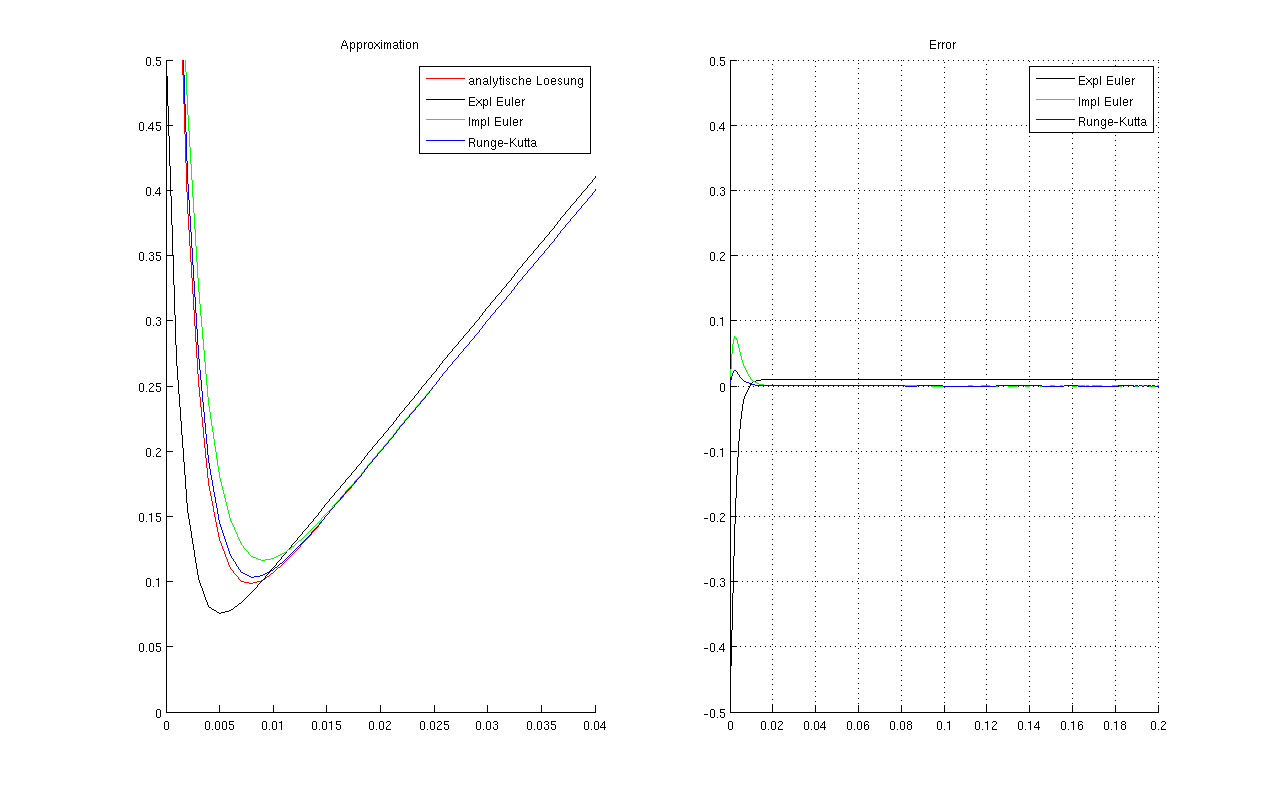
\includegraphics[width=\textwidth]{stiff0001.png}
            \caption{Stiff (h=0.001)}
            \label{pic:stuff001}
		\end{figure} 
	
	
	\begin{figure}[H]
			\centering	
			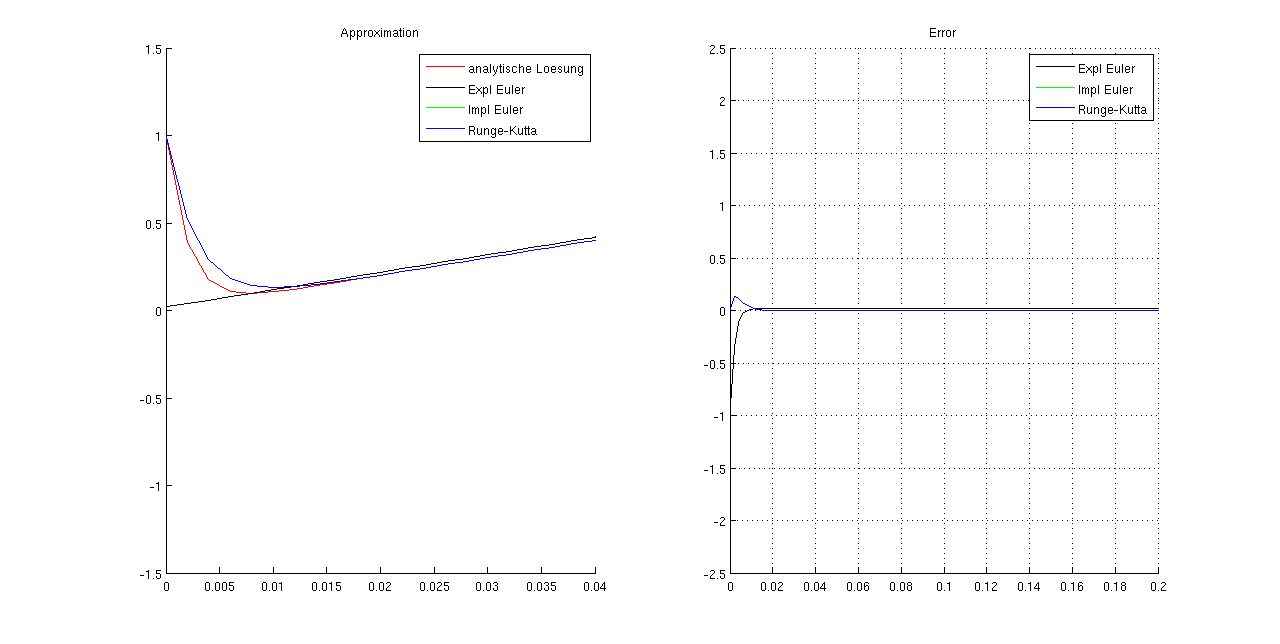
\includegraphics[width=\textwidth]{stiff0002.png}
            \caption{Stiff (h=0.002)}
            \label{pic:stuff002}
		\end{figure} 
	
	
	\begin{figure}[H]
			\centering	
			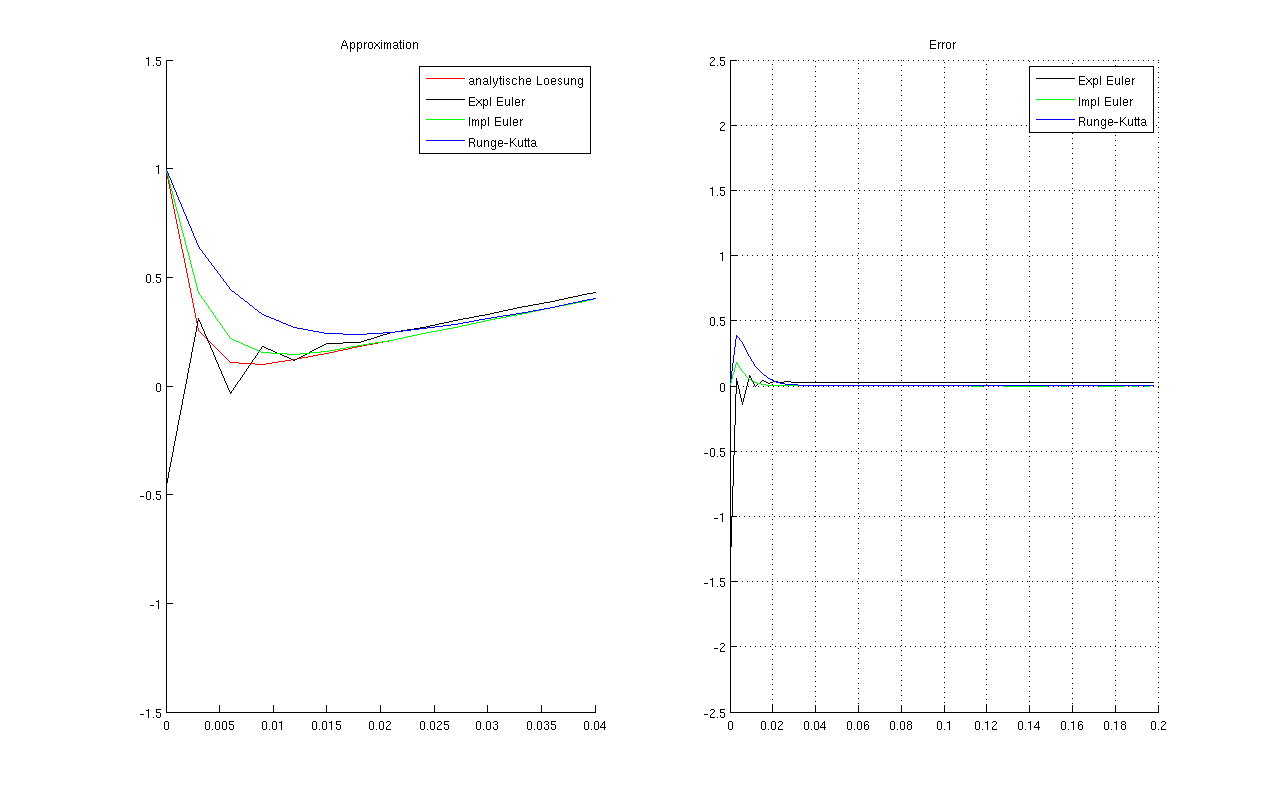
\includegraphics[width=\textwidth]{stiff0003.png}
            \caption{Stiff (h=0.003)}
            \label{pic:stuff003}
		\end{figure} 
	
	
	\begin{figure}[H]
			\centering	
			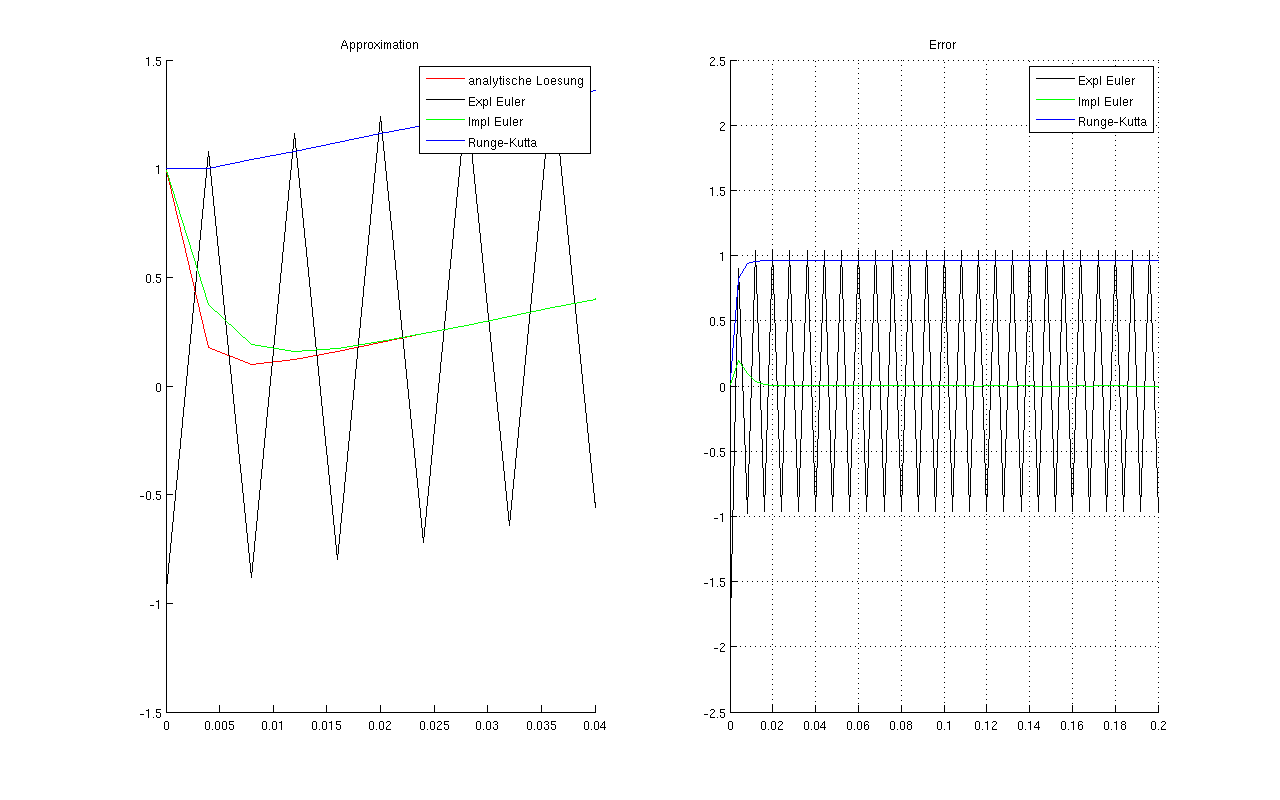
\includegraphics[width=\textwidth]{stiff0004.png}
            \caption{Stiff (h=0.004)}
            \label{pic:stuff004}
		\end{figure} 
	
	\begin{figure}[H]
			\centering	
			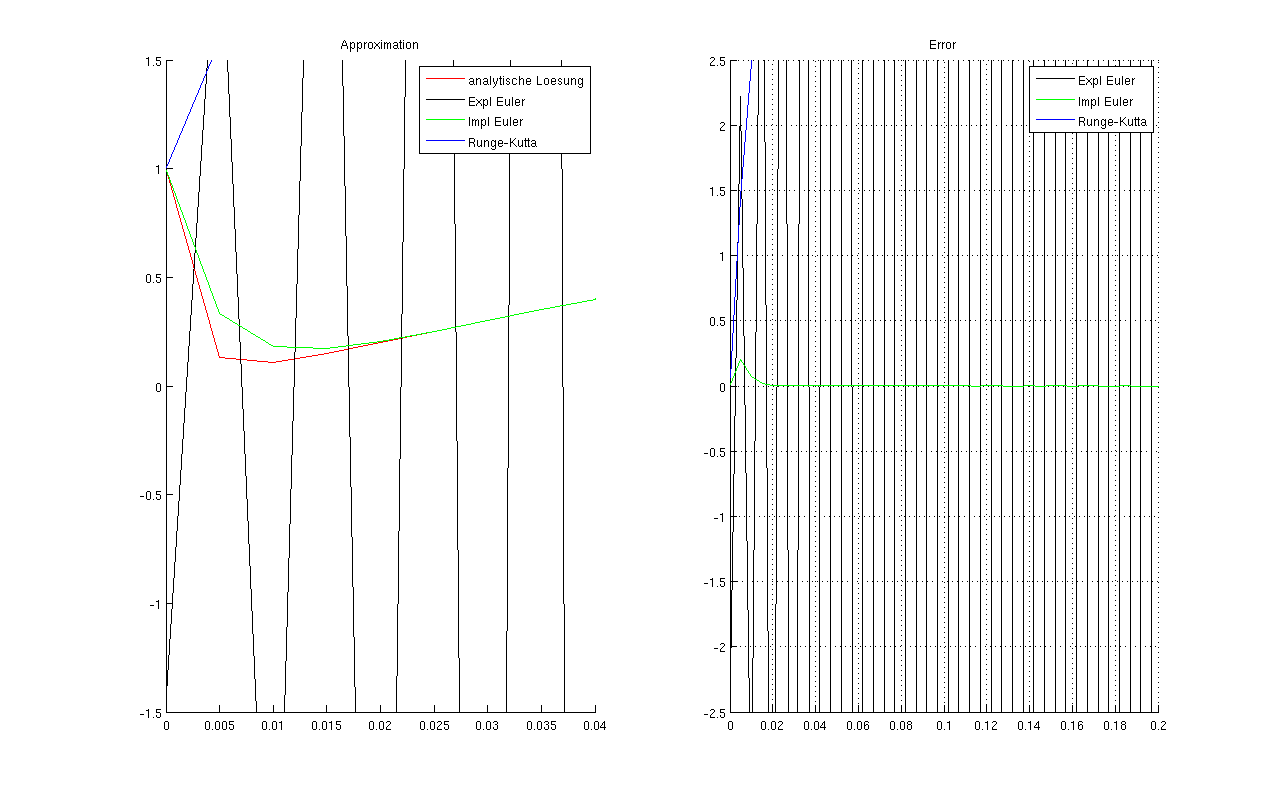
\includegraphics[width=\textwidth]{stiff0005.png}
            \caption{Stiff (h=0.005)}
            \label{pic:stuff005}
		\end{figure} 
	
	
\subsection{Ergebnisse}
	\subsubsection{h=0.001}
		\begin{figure}[H]
			\centering	
			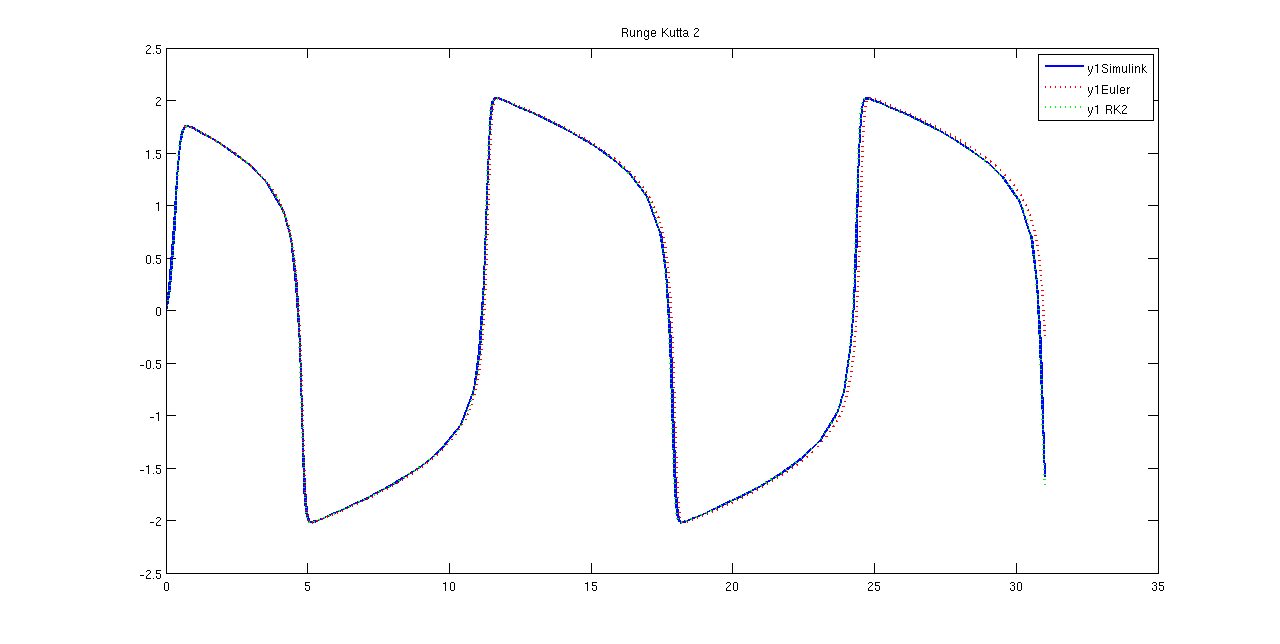
\includegraphics[width=\textwidth]{vanDerPolY10001.png}
            \caption{Van Der Pol DGL Y1 h=0.001}
            \label{pic:y2vdp0001}
		\end{figure} 
		
		\begin{figure}[H]
			\centering	
			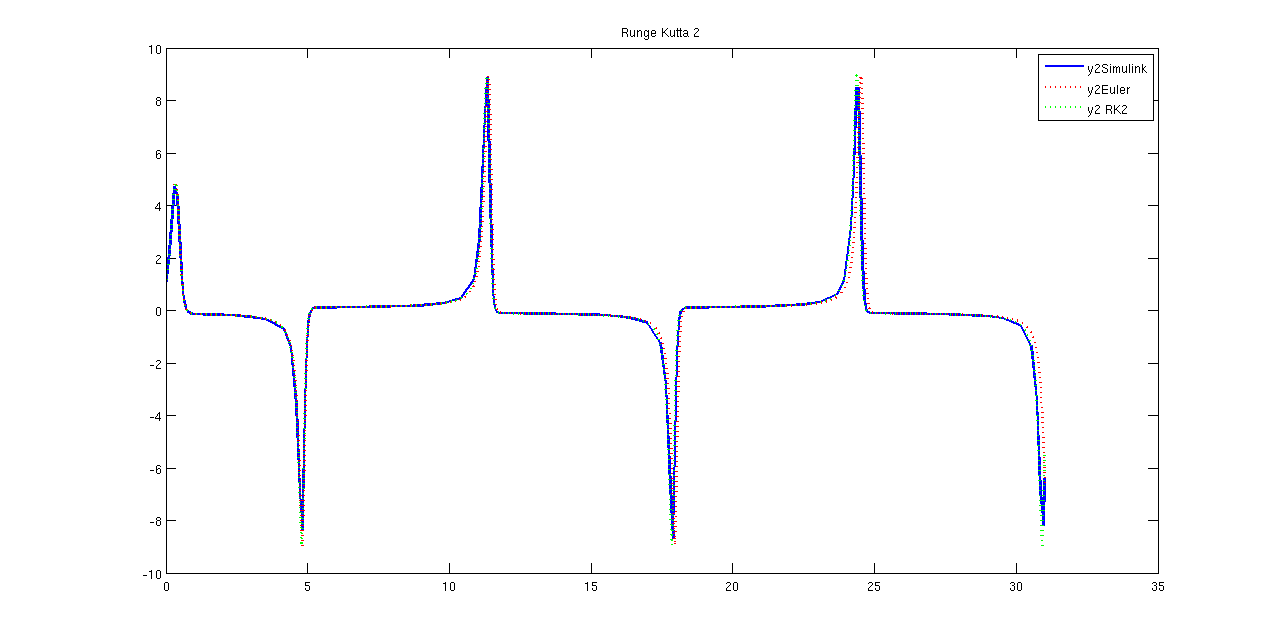
\includegraphics[width=\textwidth]{vanDerPolY20001.png}
            \caption{Van Der Pol DGL Y2 h=0.001}
            \label{pic:y2vdp0001}
		\end{figure}		
		
	Bei einer Schrittweite $h$ von $0.001$ ist zu erkennen das beide Approximationsverfahren (Expliziter Euler und Runge Kutta 2. Ordnung) mit der aus Simulink extrahierten Approximation (Dormand-Prince, Variable Step Size) übereinstimmen.
		
	\subsubsection{h=0.02}	
		\begin{figure}[H]
			\centering	
			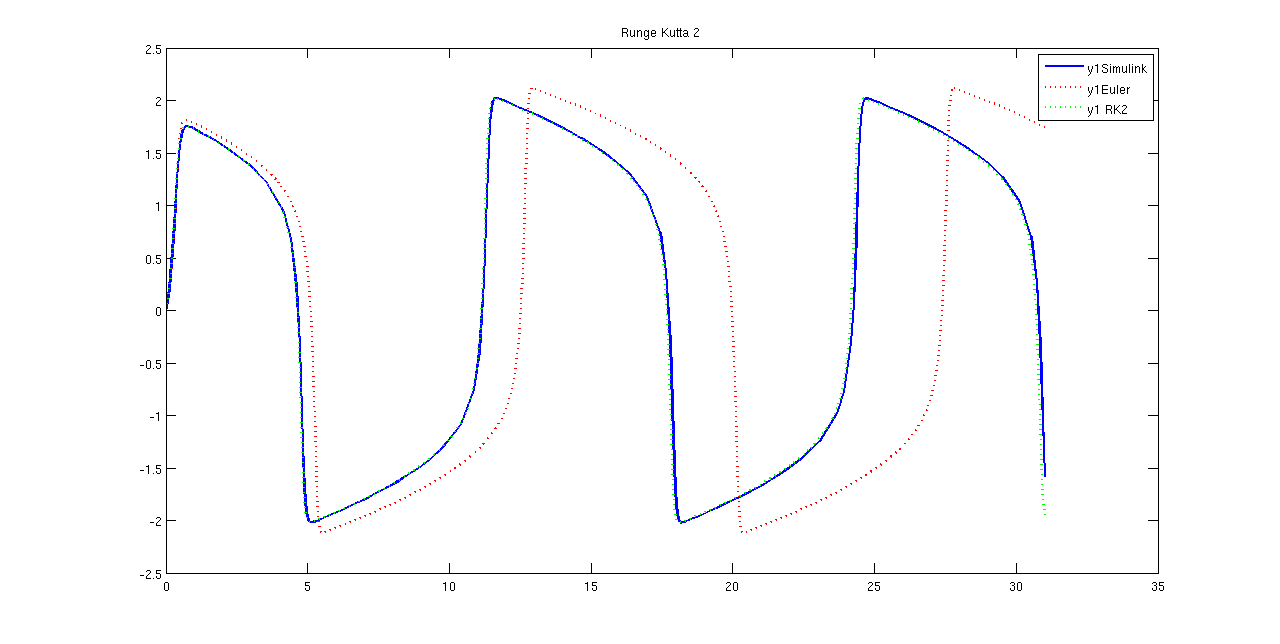
\includegraphics[width=\textwidth]{vanDerPolY102.png}
            \caption{Van Der Pol DGL Y1 h=0.02}
            \label{pic:y2vdp02}
		\end{figure} 
		
		\begin{figure}[H]
			\centering	
			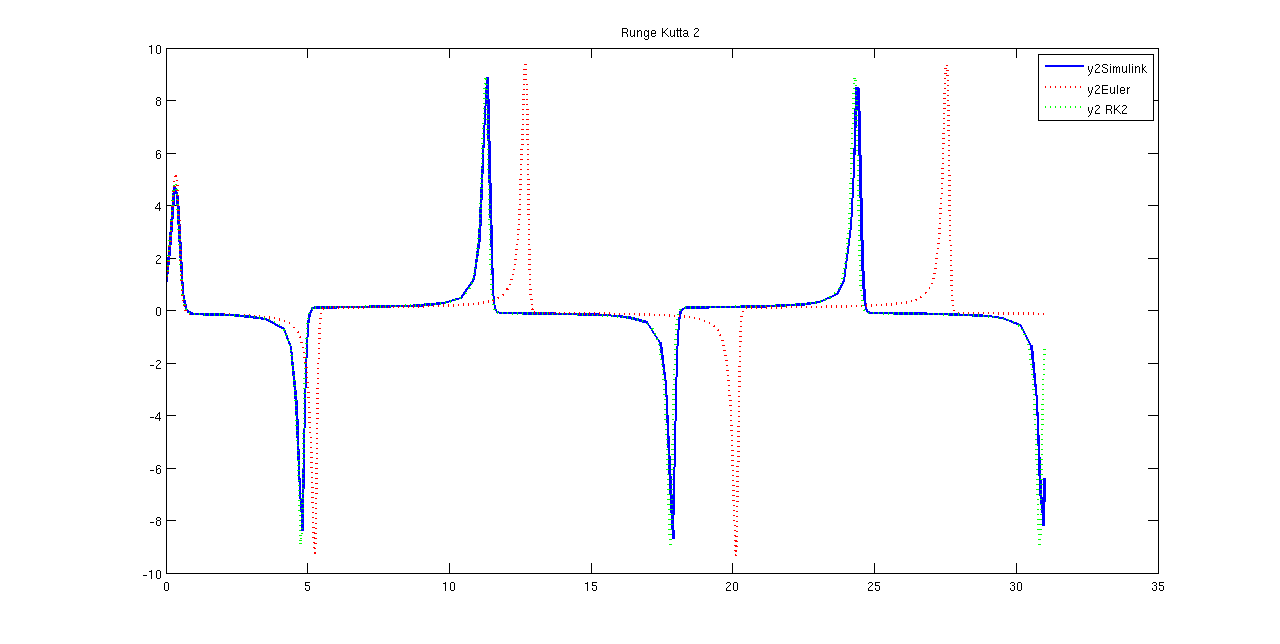
\includegraphics[width=\textwidth]{vanDerPolY202.png}
            \caption{Van Der Pol DGL Y2 h=0.02}
            \label{pic:y2vdp02}
		\end{figure}		
		
	Bei einer Schrittweite $h$ von $0.02$ ist zu erkennen das das simplere Approximationsverfahren (Expliziter Euler) deutlich von der aus Simulink extrahierten Approximation (Dormand-Prince, Variable Step Size) abweicht während das komplexere Verfahren (Runge Kutta 2. Ordnung) auch hier noch sehr dicht an Simulink liegt.
	
	\subsection{Matlab Programme}
	\lstinputlisting[tabsize=2, frame=single, label=vdp, caption={VanDerPol GDL}]{vdp.m}
	\lstinputlisting[tabsize=2, frame=single, label=vdpZeigen, caption={VanDerPol}]{vanDerPollZeigen.m}
		
	

\end{document}

